\section{Architecture}

This section will focus on the chosen architecture for our game. There exist different architecture, but we have look at the client-server model, peer-to-peer model and model view controller as possible candidates. We first describe our chosen architecture and then present the alternatives.

\subsection{Client-Server Model}
Our application will make use of the Client-Server model, a model that consists of two parts, a client and a server. The basic structure of the client-server model can be seen in \autoref{fig:client-server}.

\begin{figure}[h]
  \centering
    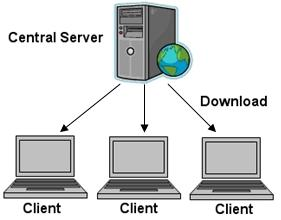
\includegraphics[width=0.5\textwidth]{img/client_server.jpg}
  \caption{Client-Server Technology \citep{ClientServer}}
  \label{fig:client-server}
\end{figure}

The client runs on the users PC, and is responsible for rendering the graphics and gameplay in the users browser.
This is done locally, without the need to connect to a server. The client will connect to the server over the internet to receive information such as leaderboard statistics. If multiplayer is implemented,\todo{Check: Is multiplayer implemented?} multiple clients could be able to play against one another by connecting to a central server. The server would then match the two or more players against each other in the same game and keep track of their individual progress. Depending on how this is implemented, the server could also be running the clients programs. This could be a relevant implementation for a multiple of reasons. One reason would be to prevent cheating. If the server executes the programs, situations where the client is modified to increase the number of points given or the time taken to solve a problem could be avoided.\todo{Other reasons?}

\subsection{Alternative Models}

\subsubsection{Peer-to-Peer}
An alternative to the Client-Server model is the Peer-to-Peer model. The Peer-to-Peer model is like the Client-Server model without the server, instead all the clients connect to each other in a decentralized system, as seen in \autoref{fig:p2p}.

\begin{figure}[h]
  \centering
    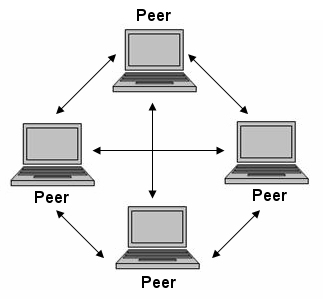
\includegraphics[width=0.4\textwidth]{img/p2p.jpg}
  \caption{Peer-to-Peer Technology \citep{PeerToPeer}}
  \label{fig:p2p}
\end{figure}

One of the positive aspects of this model is, that it drastically reduces the cost that a Client-Server based system has to keep servers running by avoiding the server completely. However, the Peer-to-Peer model also has some negative features. One of these features is that because most of the peers in a Peer-to-peer system are PC's, they may not always be available, and thus if no or few people are playing the game, it becomes difficult to play at all. Another negative feature is that the prevention of cheating becomes more difficult, since it is possible to have player clients run each others programs, but modified clients can still take over the system and corrupt the results.\newline

\subsubsection{Model-View-Controller}\todo{See \url{http://professor.unisinos.br/wp/crespo/files/2011/07/00950428.pdf}}
The Model-View-Controller design pattern separates the representation of information from a user's interaction with it. MVC is often used in web applications and consists of three separate parts, model, view, and controller. Due to the separation of data and user input, it is possible to have multiple different views for the same data. An example could be that the boss of a company should be able to access a list of all employees with their salaries, where the secretary should only have access to the list of employees without salaries. An overview of the MVC workflow can be seen on \autoref{fig:mvc}.\\

\begin{figure}[h]
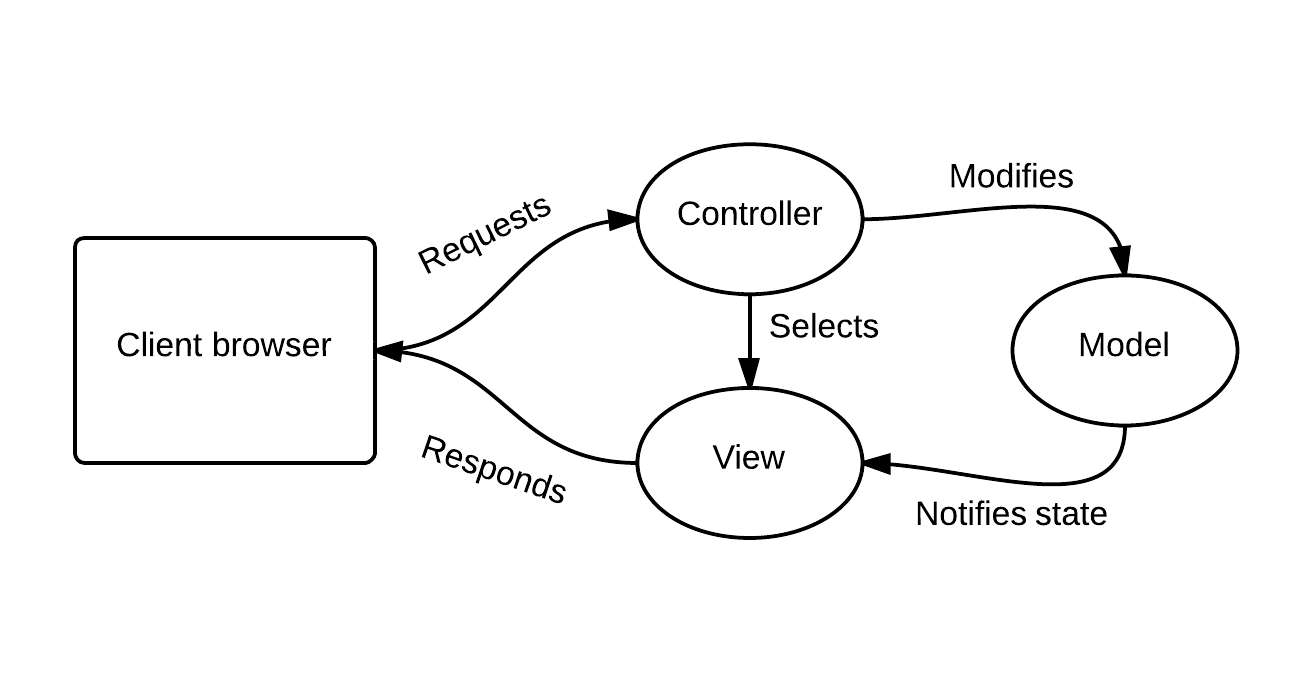
\includegraphics[width=\textwidth]{img/mvc.png}
\caption{Overview of the MVC workflow.}
\label{fig:mvc}
\end{figure}

\textbf{Model:} contains the logic, which is usually designed in such a way that it can be reused and be shared with other applications. The model ignores how user requests are issued and how data is represented to the user.\\

\textbf{View:} handles the representation of data for the end users. It is possible for an application to have multiple different views for use in various situations. The view ignores the form of user requests and the source of the data.\\

\textbf{Controller:} manages user interactions and instanciates the model and view based on performed actions, user rights and the like. The controller ignores the logic of the model and the presentation of the view.